

\documentclass[twocolumn,secnumarabic,amssymb, nobibnotes, aps, prl,superscriptaddress]{revtex4-1}
%\usepackage{acrofont}%NOTE: Comment out this line for the release version!
\newcommand{\revtex}{REV\TeX\ }
\newcommand{\classoption}[1]{\texttt{#1}}
\newcommand{\macro}[1]{\texttt{\textbackslash#1}}
\newcommand{\m}[1]{\macro{#1}}
\newcommand{\env}[1]{\texttt{#1}}
\setlength{\textheight}{9.5in}
\usepackage{amsmath}
\usepackage{amsfonts}
\usepackage{amssymb}
\usepackage[english]{babel}			
\usepackage{graphicx}
\usepackage{hyperref}
\usepackage{longtable}
\usepackage{float}
\usepackage{datetime}				% custom date
\usepackage{dsfont}					% for indicator function 1
\usepackage{circuitikz}		

\usepackage{url}					% clickable links
\usepackage{marvosym}				% symbols
\usepackage{wrapfig}				% wrapping text around figures
\usepackage[T1]{fontenc}			% font encoding
\usepackage{charter} 		

\usepackage{listings}				% for adding coloured code
\usepackage{color}
\definecolor{codegreen}{rgb}{0,0.6,0}
\definecolor{codegray}{rgb}{0.5,0.5,0.5}
\definecolor{codepurple}{rgb}{0.58,0,0.82}
\definecolor{backcolour}{rgb}{0.95,0.95,0.92}
\lstdefinestyle{mystyle}{
    backgroundcolor=\color{backcolour},   
    commentstyle=\color{codegreen},
    keywordstyle=\color{magenta},
    numberstyle=\tiny\color{codegray},
    stringstyle=\color{codepurple},
    basicstyle=\footnotesize,
    breakatwhitespace=false,         
    breaklines=true,                 
    captionpos=b,                    
    keepspaces=true,                 
    numbers=none,                    
    numbersep=5pt,                  
    showspaces=false,                
    showstringspaces=false,
    showtabs=false,                  
    tabsize=2
}
\lstset{style=mystyle}

	\newdateformat{mydate}{\monthname[\THEMONTH] \THEYEAR}


% Customize (header and) footerb
%\usepackage{fancyhdr}
%\pagestyle{fancy}
%\lfoot{	\footnotesize 
%		Mathematics Today magazine article \\
%		\Mundus\ \href{www.warwick.ac.uk/mathsys}{Mathematics for Real-World Systems CDT, University of Warwick and BT Research, Adastral Park}	\quad
		%\Telefon\ 555-5555											\quad
%\\		\Letter\ \href{mailto:R.Gowers@warwick.ac.uk}{Corresponding author: R.Gowers@warwick.ac.uk}
%	  }
%\cfoot{}
%\rfoot{\footnotesize ~\\ Page \thepage}
%\renewcommand{\headrulewidth}{0.0pt}	% no bar on top of page
%\renewcommand{\footrulewidth}{0.4pt}	% bar on bottom of page

%%% ---------------
%%% DEFINITIONS
%%% ---------------


\newcommand{\NewsItem}[1]{%
		\large #1 \vspace{4pt}
		\par \normalsize \normalfont}
		
\newcommand{\NewsAuthor}[1]{%
			\hfill \textsc{#1} \vspace{4pt}
			\par \normalfont}		


%%% ---------------
%%% BEGIN DOCUMENT
%%% ---------------
\begin{document}
% Title	
% -----

\title{Convex optimisation in communications with cvxpy}

\author{Robert P.~Gowers}%
\affiliation{Department of Mathematics, University of Warwick}
\author{Sami C.~Al-Izzi}%
\affiliation{Department of Mathematics, University of Warwick}
\author{Timothy M.~Pollington}%
\affiliation{Department of Mathematics, University of Warwick}
\author{Roger J.~W.~Hill}%
\affiliation{Department of Mathematics, University of Warwick}
\author{Keith Briggs}
\affiliation{BT, Adastral Park}

\maketitle
% -----

% Front article
% -----
	\NewsItem{``Nothing takes place in the world whose meaning is not that of some maximum or minimum.''}
	\NewsAuthor{Leonard Euler (1707-1783)}
    
\section{Introduction}
Convexity is an important property in optimisation. This is because if a problem is convex then the task of finding a global minimum is reduced to that of finding a local minimum. The importance of finding these minima efficiently in science and engineering has driven the development of software packages, such as \texttt{cvxpy}.

Here we show that many interesting problems in communications not only have a convex formulation (as shown in \cite{cvxpybook}), but can be easily implemented computationally using the \texttt{cvxpy} programming language. The ease of implementation of such problems makes \texttt{cvxpy} an invaluable tool for both students and researchers in many areas of science and engineering.
\subsection{Convex Sets and Functions}

If a set $C$ is \textit{convex}, then for any two points $x,y\in C$, any point $z$ along the $x,y$ line must also $\in C$ \cite[p.23]{cvxpybook}. More formally, for $x,y\in C$ and $\theta\in [0,1]$:
\begin{align}
\theta x + (1-\theta)y\in C.
\end{align}

In terms of a function $f$, where $f:\mathbb{R}^n \rightarrow \mathbb{R}$. For $f$ to be \textit{convex} then the domain of $f$, $\textbf{dom} f$, must be a convex set and $\forall x,y\in \textbf{dom} f$ \cite[p.67]{cvxpybook}:
\begin{align}
f(\theta x + (1-\theta)y) \leq \theta f(x)+(1-\theta)f(y).
\end{align}
This means that the function is less than or equal to linear. This can be seen graphically in Fig~\ref{fig:convex}. A concave function can be made convex by the operation $f\to-f$.
\begin{figure}
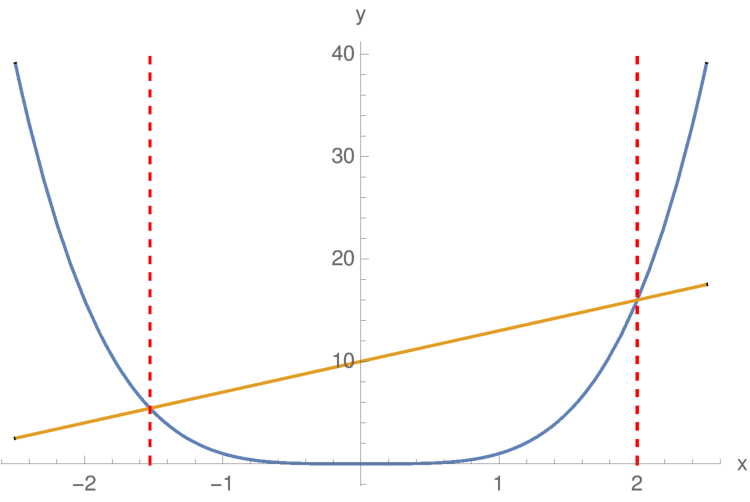
\includegraphics[width=0.9\linewidth]{convex_function.pdf}
\caption{\label{fig:convex}A chord showing convexity of the function $x^4$.} 
\end{figure}

\subsection{Convex optimisation}
A \textit{convex optimisation problem} has three components:
\begin{itemize}
\item a convex \textit{objective function} $f_0(x)$,
\item $m$ convex \textit{inequality constraint functions} $f_i(x)$,
\item $k$ convex \textit{equality constraint functions} $g_j(x)$, 
\end{itemize}
where $f,g: \mathbb{R}^n \rightarrow \mathbb{R}$ \cite[p.141]{cvxpybook}. We seek an optimum $x^*\in \mathbb{R}^n$, where $f_0(x^*)$ is a minimum. Formally the problem is defined as:
\begin{align} \label{eq:cvxdefn}
&\text{minimise } && f_0(x) & \nonumber &\\
&\text{subject to } && f_i(x) \leq 0,\quad & i\in \{1,..,m\}\nonumber &\\
& && g_{j}(x)=0,\quad & j\in \{1,...,k\} &.
\end{align}

Any local optimum $x^*$ for a convex optimisation problem is also a global optimum \cite[pp.138-139]{cvxpybook}. An optimum of a convex optimisation problem may not be unique: consider the convex function $f(x) = \text{const}$, which has line of optima $x^*$.

\subsection{Disciplined convex programming}
\texttt{cvxpy} is a symbolic programming language for \textit{Python} developed by Diamond and Boyd at Stanford\cite{cvxpy}. It uses a set of rules, called \textit{disciplined convex programming} (DCP), to determine whether a function is convex. If \texttt{cvxpy} finds that the function is convex, then interior point methods can be safely applied, which are guaranteed to find the optimal solution.

To implement DCP, the \texttt{cvxpy} package has a set of predefined functions in classes containing their curvature and sign. By only allowing certain operations with these known functions, general composition theorems from convex analysis can be applied to determine the convexity of the more complex expression. See Fig. \ref{fig:DCP}.

\begin{figure}
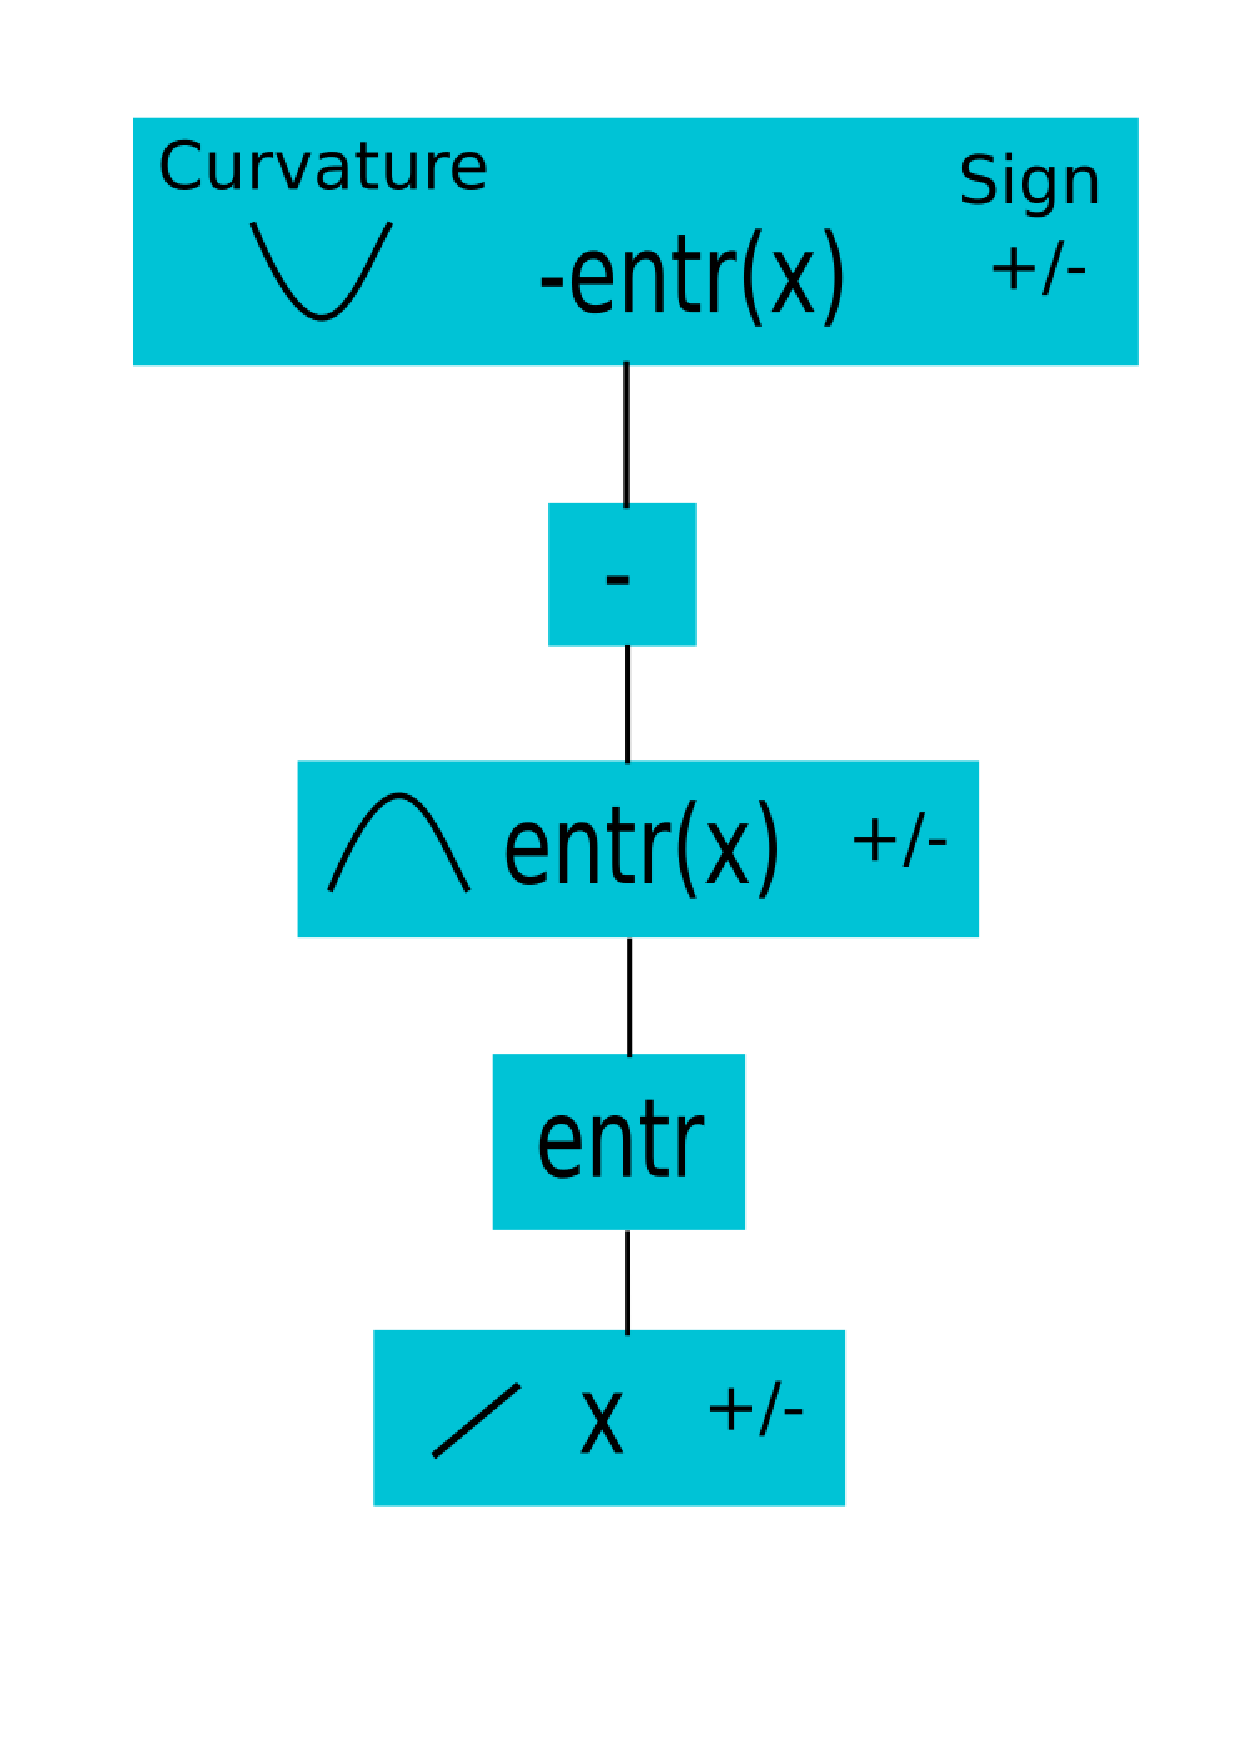
\includegraphics[width=0.7\linewidth]{DCP.pdf}
\caption{\label{fig:DCP}Application of DCP rules to a set of \texttt{cvxpy} functions, where $\text{entr}(x)=-x\log(x)$.  Figure adapted from the Stanford DCP Analyzer \cite{dcp}.}
\end{figure}

The set of available DCP functions do not define the complete set of convex functions. However, as we will show later, a large class of interesting convex problems can be written in DCP format.

We will show how \texttt{cvxpy} can be used simply to test a variety of optimisation problems, as a powerful easy-to-use tool for gaining insight into real-world problems.

\section{Real world applications}
\subsection{Water filling}
\begin{figure}
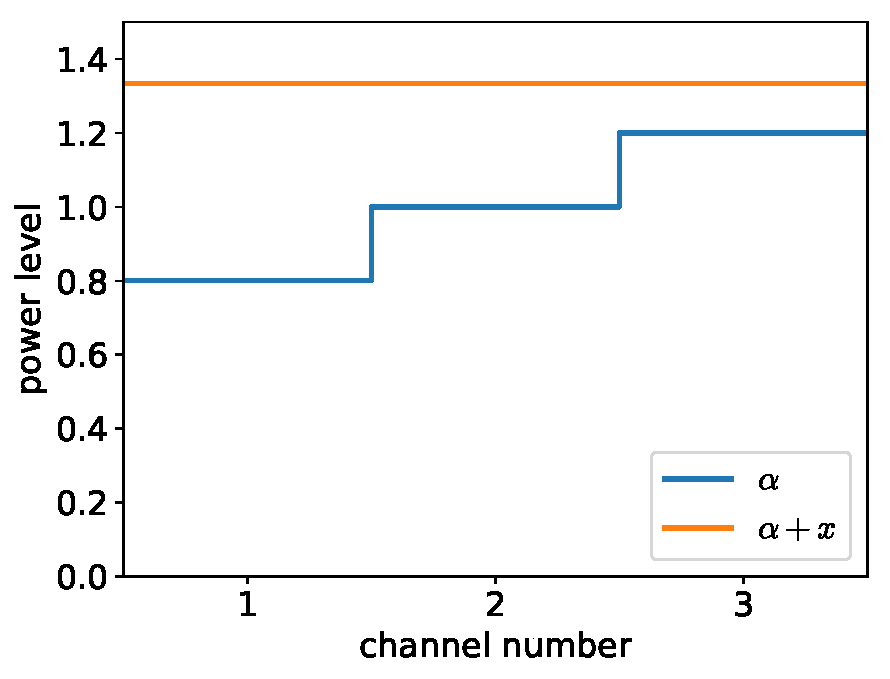
\includegraphics[width=1.0\linewidth]{water_filling_plot.pdf}
\caption{\label{fig:waterfilling}Water filling solution for three channels.}
\end{figure}

Convex optimisation can be used to solve the classic water filling problem.  In communications, this is where a total power $P$ must be assigned to $n$ different communication channels, with the objective of maximising the total communication rate.  The communication rate of the the $i$th channel, $r_i$, is given by \cite[p.245]{cvxpybook},

\begin{align}
r_i = \log(x_i+\alpha_i),
\end{align}
where $x_i$ is the power allocated to channel $i$ and $\alpha_i$ represents the floor above the baseline at which power can be added to the channel.  From Fig. \ref{fig:waterfilling}, we can see how this is analogous to filling an uneven basin to a constant level. 

%Consider a bounded area of contiguous, equal-area patches $i$ of different elevations $\alpha_i$ (Fig.~\ref{fig:waterfilling}). The area is flooded to a certain level. Find the optimal height $x^{*}_i$ that uses a total amount of water of 1---this describes the famous `water filling' (or `water pouring') problem. It is also common to information theory, formulated by allocating power to communication channels, where each transmits at power $p_i$ and bandwidth $\alpha_i$, with channel rate $\log(\alpha_i+p_i)$\cite[p.245]{cvxpybook}.

The optimisation problem is then \cite{cvxpybook}:
\begin{align}
& \text{minimise} 
& & f_{0}(\textbf{x})=-\sum^{n}_{i=1}\log(\alpha_{i}+x_{i}),\quad\boldsymbol{\alpha} \succ \textbf{0}\nonumber\\
& \text{subject to} 
&& \textbf{x} \succeq \textbf{0} , \nonumber\\& && \sum^{n}_{i=1}x_{i}=\mathds{1}^{T}\textbf{x}=P
\end{align}
where symbols $\succ$, $\succeq$ denote elementwise inequalities between vectors or matrices. 

This is a convex problem since $f_0(\textbf{x})$ has positive curvature within its domain, and the inequality and equality constraints are convex. 

\subsubsection{Example \texttt{cvxpy} code in Python}
To indicate the brevity of code implementation in \texttt{cvxpy} we show an abridged version below:
\lstinputlisting[language=Python]{waterfilling.py}

\subsubsection{Computational complexity}
\texttt{cvxpy} employs different solvers for each problem and so they have different computational complexities; these were assessed by averaging the runtime over many runs.\\ 
In the case of water filling, for problem sizes up to 1000 channels, the computational time scaled linearly, Fig.~\ref{fig:waterfillingcomputcomplex}.Given that we have $n$ items in this problem and we apply the objective function to each channel independently, a computational complexity of $O(n)$ should be expected.

\begin{figure}
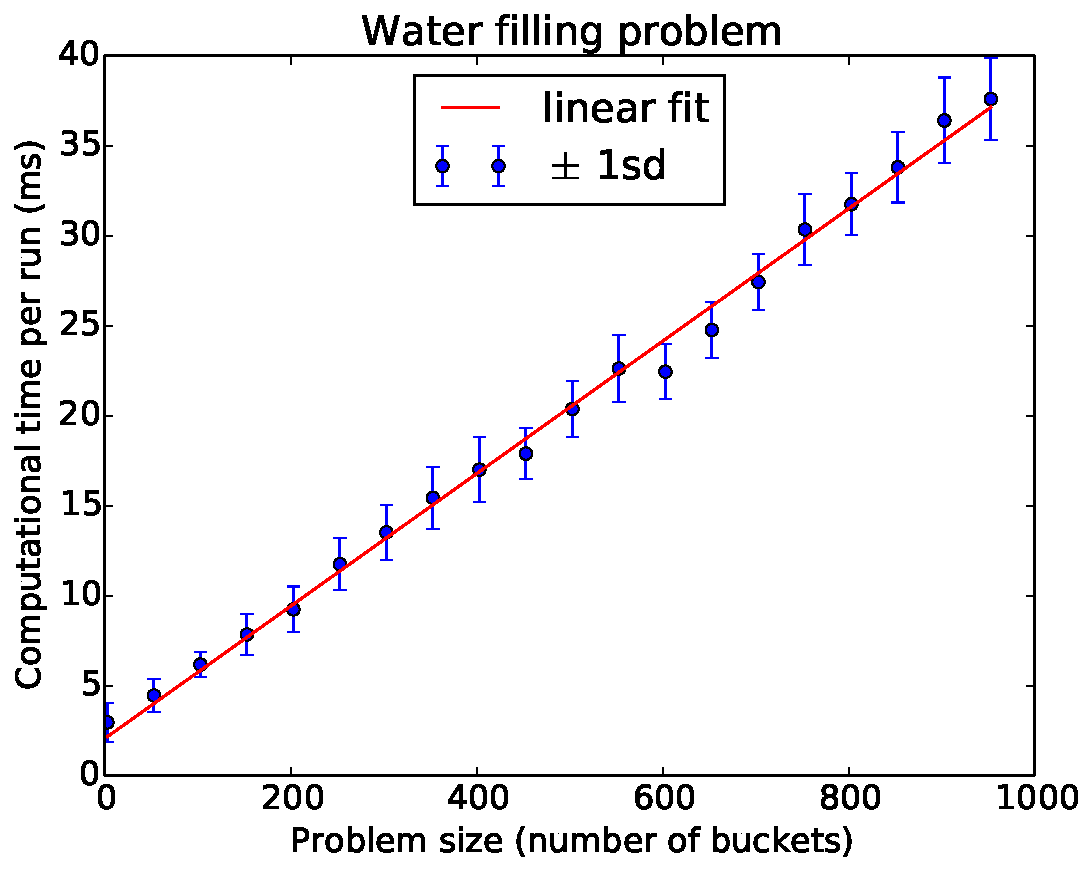
\includegraphics[width=0.9\linewidth]{water_filling_1000runs_1000buckets.pdf}
\caption{\label{fig:waterfillingcomputcomplex}Linear plot of computation time (wall time) of water filling against problem size, for 1000 runs.}
\end{figure}

\subsection{Maximising channel capacity}

Convex optimization can be used to find the channel capacity $C$ of a discrete memoryless channel. Consider a communication channel with input $X(t)\in\{1,2,...,n\}$ and output $Y(t)\in\{1,2,...m\}$. This means that the random variables $X$ and $Y$ can take $n$ and $m$ different values respectively.

In a discrete memoryless channel, the relation between the input and the output is given by the transition probability,
\begin{equation}
p_{ij} = \mathbb{P}(Y(t)=i|X(t)=j),
\end{equation} where these transition probabilities form the channel transition matrix $P$, with $P \in \mathbb{R}^{m\times n}$.  Assume that $X$ has a probability distribution denoted by $x\in\mathbb{R}^n$, meaning that,
\begin{equation}
x_j = \mathbb{P}(X(t) = j), \quad j=\{1,...,n\}.
\end{equation}
From Shannon \cite{shannon1949}, the channel capacity is given by the maximum possible mutual information, $I$, between $X$ and $Y$,
\begin{align}
C &= \sup_x I(X;Y), \quad \text{where},\\
I(X;Y) &= -\sum_{i=1}^{m}y_i\log_2 y_i+\sum_{j=1}^{n}\sum_{i=1}^{m}x_j p_{ij}\log_2 p_{ij}.
\end{align}

Given that $x\log x$ is convex for $x\geq 0$, we can formulate this as a convex optimisation problem,
\begin{align}
\text{minimise} \quad -I(X;Y), \\
\text{subject to} \quad \sum_{i=1}^{n}x_i = 1, \quad x \succeq 0.
\end{align} Here the constraints arise from $x$ describing a probability.

\subsubsection{Example \texttt{cvxpy} code}
Due to the built-in entropy function in \texttt{cvxpy}, \texttt{cvx.entr()}, the channel capacity problem is easy to write in DCP.

\lstinputlisting[language=Python]{channel_capacity.py}

\subsubsection{Computational complexity}
The computational complexity of the channel capacity problem follows a power law in \texttt{cvxpy}.  For $n$ up to 1000, the complexity is of order $\sim O(n^{2.5})$, Fig.~\ref{fig:channel_capacity_complexity}. Given that we are applying matrix multiplication to the power vector $\textbf{p}$, a complexity of at least $n^2$ would be expected.
\begin{figure}
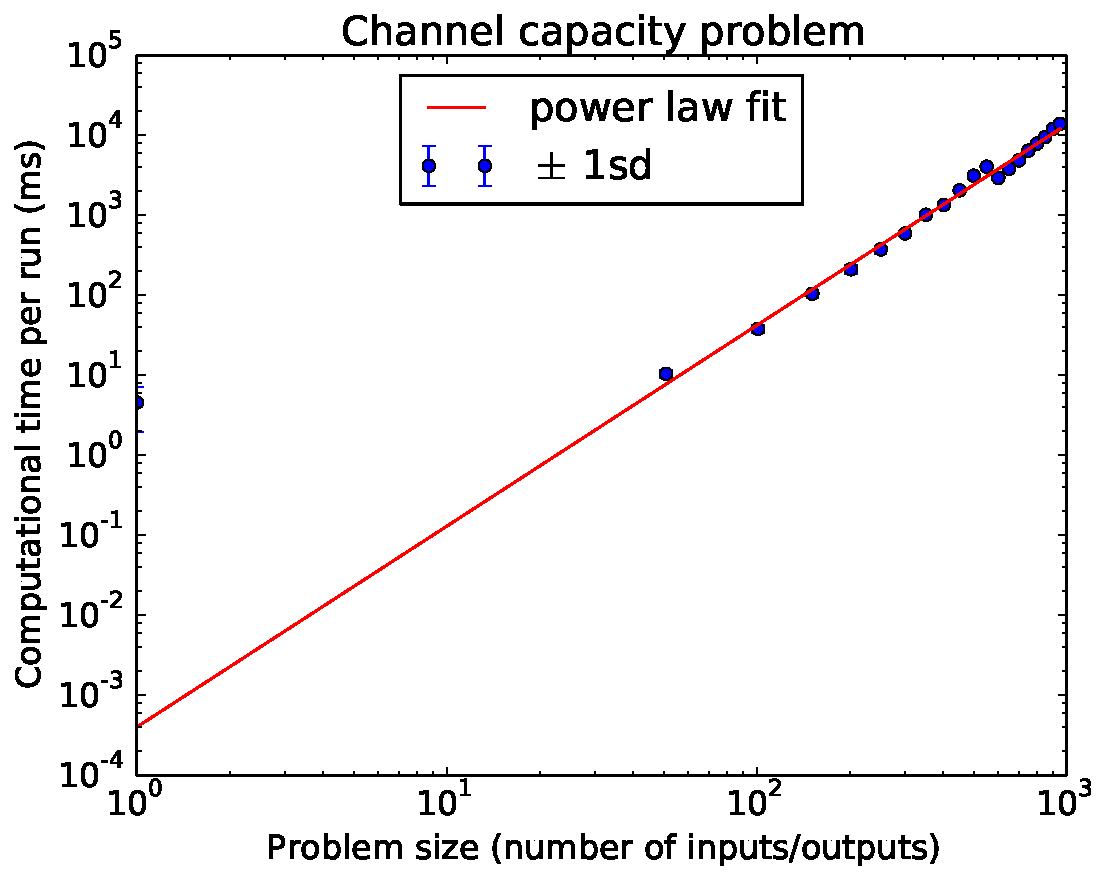
\includegraphics[width=0.9\linewidth]{channel_capacity_complexity.pdf}
\caption{\label{fig:channel_capacity_complexity}Log-log plot of computation time (wall time) of channel capacity against problem size, for 1000 runs.}
\end{figure}

\subsection{Minimum power for a given SINR}
How can we minimise the total power consumption $P$ of $n$ transmitters each with power $p_i$, yet achieve a minimum SINR $\gamma_0$ for all $m$ receivers? This question is relevant to a telecoms company who want to offer a service at a minimum quality standard. We formulate the problem with a given square path gain matrix $G$, background noise level $\sigma$ and maximum power value that any transmitter can reach $P_{\text{max}}$:
		\begin{align*}
				&\underset{p}{\text{minimise}} \quad &&\sum_j p_j\\
				&\text{subject to} \quad &&p_j \leq P_{\max}\\
				& \quad &&p_j \geq 0\\
				& \quad &&\gamma_i \geq \gamma_0&&
		\end{align*}
The desired signal to receiver $i$ is denoted by $S_i = G_{ik}p_k$, while the interference to $i$ is $I_i = \sum_{j\neq k}G_{ij}p_j$. However DCP does not allow division of the optimisation variable $p_i$ so  
\begin{equation*}
  \gamma_i \geq \gamma_0\Longleftrightarrow  \frac{S_i}{\sigma_i + I_i}\geq \gamma_0, \quad \forall i
\end{equation*}
was rearranged to:
\begin{equation*}
S_i-\gamma_0(\sigma_i + I_i)\geq 0, \quad \forall i
\end{equation*} which is DCP.
\subsubsection{Path gain}
The path gain $G_{ij}$ represents the proportion of power that reaches receiver $i$ from transmitter $j$. Supposing that the desired signal to receiver $i$ is from transmitter $k$, the power received is,
\begin{equation}
p_{ik}^{\text{rec}} = G_{ik}p_k.
\end{equation}
The signal-to-interference-plus-noise ratio (SINR) is the strength of the desired signal $S_i$ relative to the interference power $I_i$ plus the background noise $\sigma_i$ at $i$. Denoting the SINR at $i$ by $\gamma_i$, we have
\begin{equation}
\gamma_i = \frac{G_{ik}p_k}{\sigma_i+\sum_{j\neq k}G_{ij}p_j}
=\frac{S_i}{\sigma_i+I_i}.
\end{equation}

In a physical context, the path gain from transmitter $j$ to receiver $i$ will depend on the distance, $d_{ij}$ between them.  Assuming isotropic propagation from each transmitter, the fraction of power from $j$ that reaches $i$ is given by,

\begin{equation}
G_{ij} = k_i/d_{ij}^\alpha
\end{equation}

where $\alpha$ is the pathloss coefficient, $k$ is a proportionality constant specific to the receiver $i$.  For free space $\alpha = 2$, while for an urban environment $\alpha \sim 3.5$.  Further physical complexities, such as the stochastic effects from Rayleigh fading can be easily implemented.

\begin{figure}[H]
\centering
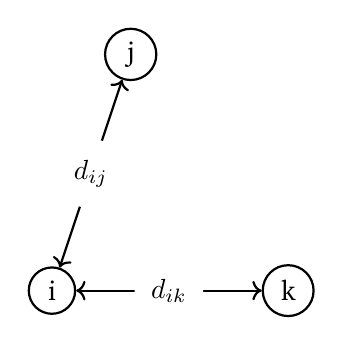
\begin{tikzpicture}
\begin{scope}[every node/.style={circle,thick,draw}]
    \node (A) at (0,0) {i};
    \node (B) at (1,3) {j};
    \node (C) at (3,0) {k};
\end{scope}
\begin{scope}[
	every node/.style={fill=white,circle},
    every edge/.style={draw=black, thick}]
    \path [<->] (A) edge node {$d_{ik}$} (C);
    \path [<->] (B) edge node {$d_{ij}$} (A);
    %\path [<->] (C) edge node {$1$} (B);
\end{scope}
\end{tikzpicture}
\caption{Path lengths between receiver $i$ and transmitters $j$ and $k$.}\label{fig:spatial_diagram}
\end{figure}

\subsubsection{Example code}
The \texttt{cvxpy} implementation is shown below.
\lstinputlisting[language=Python]{minimisePgivenSINR.py}

\subsubsection{Computational Complexity}

\begin{figure}[H]
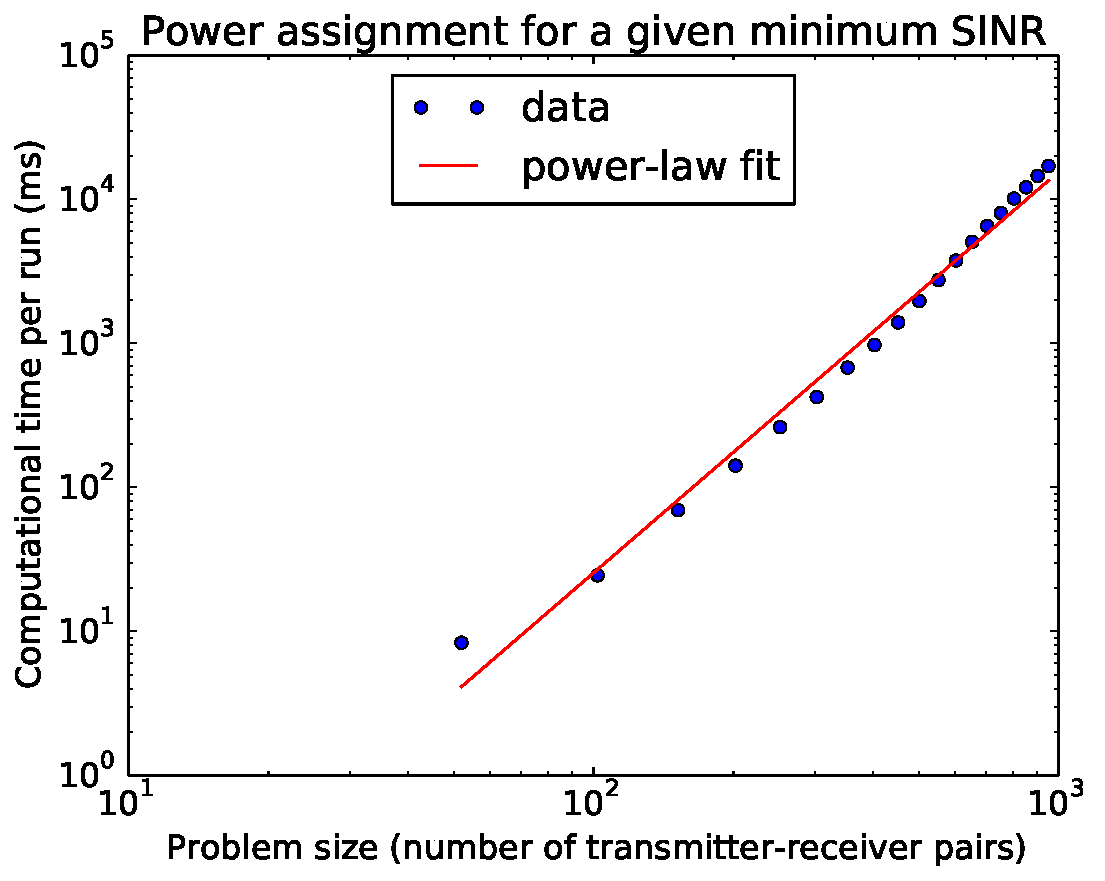
\includegraphics[width=0.9\linewidth]{magazineMinSINR.pdf}
\caption{\label{fig:MinSINR}Log-log plot of computation time (wall time) of minimum power problem against the problem size, for 25 runs.}
\end{figure}

The computational complexity of the power minimisation for $n$ up to 1000 is of order $\sim O(n^{2.8})$.

\section{Conclusions}
This article has shown that many well-known convex problems in communications can be written in a DCP format, meaning that they can be easily implemented in \texttt{cvxpy}.

Our example code demonstrates a key strength of \texttt{cvxpy}, which is that the translation from the mathematical description to python code is straightforward and clear.  Conversely, one can also infer the mathematical problem from reading the code.

The computational complexity of the problems examined had a clear trend which aligned with expectation.  This shows that convex optimisation solvers are robust to a variety of problem sizes and are scalable to at least problems of size 1000.

While all problems that can be written in DCP are convex, not all convex problems of interest can be written in DCP.  Over time, the library of available DCP functions in \texttt{cvxpy} has grown, increasing the scope of convex optimisation problems that \texttt{cvxpy} can solve.  This expansion of scope of \texttt{cvxpy} is ongoing, with version 1.0 under development and expected in the near future.

%\section{Further Work}
%While many problems are convex, others fall into a similar category of being \textit{quasi-convex}.  A quasi-convex function $f$ is one for which $\textbf{dom} f$ and every sublevel set of $f$ is convex.  An example of this is shown in Figure [?].  Quasi-convex problems cannot be solved directly using convex optimisation solvers, however the feasibility of a sublevel set can be checked.  This feasibility check can be used as a bisection method to find the solution.  A more thorough discussion of quasi-convex problems can be found in \cite{cvxpybook}chapter?.

%\section{Further applications}
\subsection*{Acknowledgements}
We would like to thank S. Johnson and S. Diamond for helpful discussions.

\section*{Appendix}
Full code can be found at\\ https://github.com/cvxgrp/cvxpy/tree/master\\/examples/communications.

\vspace{1cm}
%\section{Links \& references}
\bibliography{articleBib} 
\bibliographystyle{plain}

%\item DCP analyser http://dcp.stanford.edu/analyzer
% -----
\end{document}
